\section{Warstwa konwolucyjna}
Warstwa konwolucyjna jest podstawowym budulcem modeli, które
są wykorzystywane przez nas w tym projekcie: ResNet-ów (ang.
Residual Networks) oraz sieci InceptionTime. Wykorzystywana jest
ona przede wszystkim do pracy nad obrazami, ale może być również
stosowana przy przetwarzaniu sygnałów, takich jak sygnały EKG badane
przez nas. Warstwy te posiadają wiele zalet, które sprawiają, że
są one idealnym wyborem do pracy z naszymi danymi. Przede wszystkim,
w przeciwieństwie do warstw gęstych (warstwy w sieciach MLP), pozwalają
one na wzięcie pod uwagę lokalnych zależności danych wejściowych,
co jest kluczowe przy pracy z sygnałem takim jak EKG. Ponadto, warstwy
te mają znacznie mniej parametrów, co pozwala na szybsze uczenie,
a także zmniejsza ryzyko przeuczenia modelu.
\\

Warstwa konwolucyjna opiera się jak sama nazwa wskazuje na
operacji konwolucji. W jednym wymiarze, operacja ta polega
na przekształceniu wektora wejściowego $x$ w wektor wyjściowy $y$, tak że
każdy element $y_i$ jest obliczany jako iloczyn skalarny fragmentu wektora
wejściowego $x$ z wektorem wag $w$, który jest przesuwany po całym wektorze wejściowym.
Wzór na obliczenie elementu $y_i$ wygląda następująco:
\begin{equation}
  y_i = \sum_{j=0}^{k-1} w_j x_{i+j}
\end{equation}
Gdzie $[w_0, w_1, ..., w_{k-1}]^T$ to wektor wag, a $k$ to rozmiar jądra konwolucyjnego (ang. kernel size).
\\

Spójrzmy sobie teraz na parametry warstwy konwolucyjnej, które będziemy
wykorzystywać w dalszej części.
\begin{figure}[H]
  \centering
  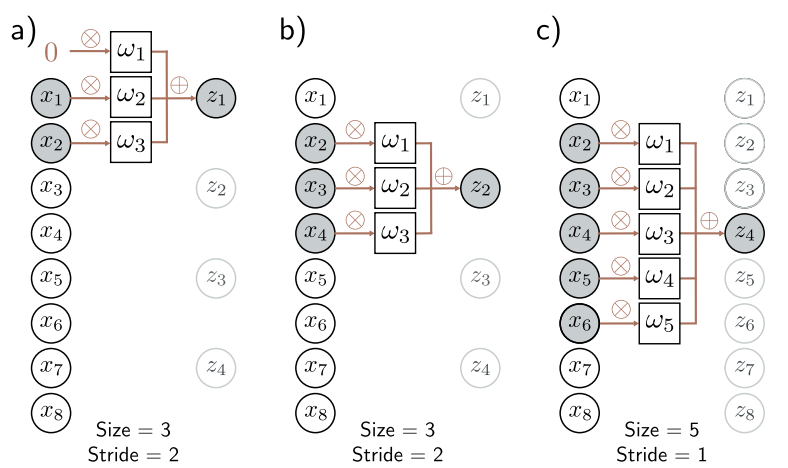
\includegraphics[width=0.8\textwidth]{Sieci_Konwolucyjne/conv1d.png}
  \caption{Parametry warstwy konwolucyjnej. Źródło: adaptacja rysunku z \cite[s.~164]{prince2023understanding}.}
  \label{fig:conv1d}
\end{figure}

\begin{itemize}
  \item \textbf{Kernel size} - rozmiar jądra konwolucyjnego, czyli długość wektora wag, który jest
    przesuwany po wektorze wejściowym. Różna długość jądra pozwala na wychwycenie bardziej lokalnych
    (mały rozmiar jądra) lub bardziej globalnych (duży rozmiar jądra) zależności
  \item \textbf{Stride} - ten parametr określa o ile pozycji wektora wejściowego przesuwane jest jądro
    konwolucyjne podczas obliczania kolejnych elementów wektora wyjściowego

  \item \textbf{Padding} - ten parametr określa, czy i ile zer jest dodawanych do wektora wejściowego
    na początku i końcu. Pozwala on zachować rozmiar wektora wyjściowego równy rozmiarowi wektora wejściowego
    (bo zarówno kernel size, jak i stride mogą powodować zmniejszenie tego rozmiaru)
  \item \textbf{Channels (In oraz Out)} - parametr ten określa liczbę kanałów wejściowych oraz wyjściowych.
    Liczba kanałów wejściowych określa, ile różnych wektorów wejściowych jest przetwarzanych przez warstwę. Natomiast
    liczba kanałów wyjściowych określa, ile różnych wektorów wyjściowych jest generowanych przez warstwę. Liczba wag, dla
    danej warstwy jest równa $kernel\_size \times in\_channels \times out\_channels$
\end{itemize}
